\documentclass[specialist,subf,href,colorlinks=true,14pt
%,fixint=false
,times,mtpro,specialist
]{disser}
\usepackage[
  a4paper, mag=1000, includefoot,
  left=3cm, right=1.5cm, top=2cm, bottom=2cm, headsep=1cm, footskip=1cm
]{geometry}
\usepackage[T2A]{fontenc}
\usepackage[utf8]{inputenc}
\usepackage[english,russian]{babel}
\usepackage{graphicx}
\ifpdf\usepackage{epstopdf}\fi
\sloppy

\usepackage{cite,enumerate,float}

\usepackage{vmargin}
\usepackage{indentfirst}
\usepackage[T2A]{fontenc}
\usepackage{graphics}
\usepackage{amsthm}
\usepackage{amsbsy}
\usepackage{amsmath}
\usepackage{amssymb}
\usepackage{amsfonts}
\usepackage{mathtext}
\usepackage{hhline}
\usepackage{longtable}
\usepackage{fancybox,fancyhdr} 
%\usepackage{mathtext}
%\usepackage{mathenv}
%\usepackage{array}
%\usepackage{xcolor}
%\usepackage{float}
%\parindent = 30pt
%\hoffset = 12pt
%\voffset = 0pt
%\oddsidemargin = 0pt
%\evensidemargin = 0pt
%\topmargin = 9pt
%\headheight = 0pt
%\headsep = 24pt
%\textheight = 650pt
%\textwidth = 450pt
%\marginparsep = 0pt
%\marginparwidth = 9pt
%\footskip = 30pt

\begin{document}
\begin{titlepage} \newpage 
\begin{center} МОСКОВСКИЙ ГОСУДАРСТВЕННЫЙ УНИВЕРСИТЕТ\\ ИМ. М.В. ЛОМОНОСОВА\end{center} 
\vspace{8em} \begin{center} 
\Large Механико-математический факультет \\ \end{center}
\vspace{2em} \begin{center} 
\textsc{Курсовая работа \linebreak \textbf{Реализация параллельной записи больших файлов с вещественными числами в текстовом представлении}
\linebreak \linebreak \textbf{}} \end{center}
\vspace{6em} \newbox{\lbox} \savebox{\lbox}{\hbox{Я.Нагорных}} 
\newlength{\maxl} \setlength{\maxl}{\wd\lbox} \hfill\parbox{12	cm}
{ \hspace*{7.5cm}\hspace*{-5cm}Студент 4 курса:\hfill\hbox to\maxl{Нагорных Я.В.}\\
\hspace*{7.5cm}\hspace*{-5cm}Научный руководитель:\hfill\hbox to\maxl{Богачев К.Ю.}}\\  \vspace{\fill}
\begin{center} Москва \\ 2018\end{center} \end{titlepage}

%\maketitle

%\renewcommand{\contentsname}{Содержание}
\tableofcontents

\renewcommand{\figurename}{Рисунок}
\newcommand{\class}{\textcolor[rgb]{0.5,0,0.5}}
\newcommand{\type}{\textcolor[rgb]{0.5,0.5,0}}
\newcommand{\field}{\textcolor[rgb]{0.5,0,0}}

\newpage

\section*{Введение}
\addcontentsline{toc}{section}{Введение}
\paragraph{Постановка проблемы.}
Печать большив массивов чисел всегда занимает много времени.
Однако, не вся печать упирается в ресурсы диска, как это может показаться.


Кроме того, у печати данных мало ресурсов для ускорения.

Печать чисел с плавающей запятой также является проблемой, так как само значение числа и его экспоненту нельзя обрабатывать независимо. 

Стандартный подход недостаточно точен и в некоторых случаях дает неверные результаты. 
Кроме того использование функций стандартных библиотек (\texttt{printf}, \texttt{sprintf}) достаточно затратно по времени.

\textbf{Цели работы:}
\begin{enumerate}
\item Ускорить печать больших массивов;
\item Использовать быстрые алгоритмы печати целых чисел и чисел с плавающей точкой.
\end{enumerate}


Как уже было сказано, у печати массивов мало ресурсов для ускорения.
Также проблемой является и то, что печать данных файл должна быть строго последовательной, поэтому нельзя ''простым'' образом использовать распараллеливание.

Однако, известно что большую часть времени занимает преобразование типа \texttt{\type{int}} или \texttt{\type{double}} в буффер типа \texttt{\type{const char} *} непосредственно для печати.
Именно это можно и распараллелить, используя многопоточное программирование.
Непосредственно печать в сам файл упирается в возможности диска. 
Ее ускорить нельзя.

Кроме того, можно заменить стандартный алгоритм преобразования числа в строку, на более быстрые.
Мы будем использовать алгоритм \textsf{Grisu2} для печати вещественных чисел и \textsf{SSE2} для печати целых чисел, о которых будет рассказано позже.
\paragraph{Обзор предфдущих решений.}
\paragraph{Возможные варианты улучшений.}
Мы уже обратили внимание на то, что стандартная функция \texttt{sprintf (char *, const char *, \dots)} работает крайне долго. 
Возникает идея применения более быстрых алгоритмов преобразования чисел в строки. 
Так например быстрое логарифмирование (разбиение числана цифры) может ускорить процесс.

Другой идеей для улучшения является использование многопоточного программирования. 
Из-за того что печать в файл должна быть строга последовательной, кажется что ресурсов для распараллеливания немного.
Но

После того, как мы добъемся ускорения, можем использовать улучшения, которые будут оптимизировать алгоритм. 
Так например, мы можем уменьшить размер выходного файла.
Если будет встречаться несколько подряд одинаковых чисел, то можно сократить запись.
Также, немного уменьшит размер файла отбрасывание ненужных нулей в концце записи числа (после точки).


\section{Описание алгоритма}
Схематично работа алгоритма показана на Рисунке \ref{draw}.
\begin{figure}[h!]
\begin{footnotesize}
\def\svgwidth{430pt}
  \input{drawing.pdf_tex}
  \caption{Работа потоков.} \label{draw}
\end{footnotesize}\end{figure}

\subsection{Используемые структуры и классы}
\paragraph{Структура \texttt{\class{reduce\_chunk}}.}
В ней находится строковый буффер (готовый для печати) и его порядковый номер (\texttt{\field{chunk\_id}}).
Кроме того, хранится флаг, является ли этот \texttt{\class{reduce\_chunk}} последним.
\paragraph{Структура \texttt{\class{map\_chunk}}.}
Этот тип состоит из лямбда-функии, которая должна обработать определенный фрагмент массива чисел, и элемента типа \texttt{\class{reduce\_chunk}}, возвращаемый функцией.
\paragraph{Класс \texttt{\class{mutex\_wait\_queue}}.}
Это реализация \textit{блокирующей очереди}, или \textit{мьютексной очереди}.  
Под ней понимается очередь со следующим свойством: когда поток пытается прочитать что-то из пустой очереди, то он блокируется, до тех пор, пока какой-нибудь другой поток не положит в нее элемент.
У этой очереди есть следующие методы:
\begin{itemize}
\item \texttt{dequeue} -- достает верхний элемент из очереди, если очередь непустая.
Иначе, поток, вызвавший этот метод блокируется. Также можно передать время блокировки, по истечении которого, поток разблокируется и вернется ни с чем;
\item \texttt{dequeue\_all} -- аналогично \texttt{dequeue}, но достает все элементы, находящиеся в очереди, и складывает в указатель вектор из них;
\item \texttt{enqueue} -- складывает элемент в конец очереди.
\end{itemize}
\paragraph{Класс \texttt{\class{worker\_thread}}.}
Это главный управляющий поток.
Он хранит две блокирующие очереди \texttt{\field{m\_map\_queue}} и \texttt{\field{m\_reduce\_queue}}, состоящие из \texttt{\class{map\_chunk}} и \texttt{\class{reduce\_chunk}} соответственно. 
Зачем нужны такие очереди будет сказано позже.

\subsection{Распределение задач}
Управляющий (главный) поток \texttt{\class{worker\_thread}} вызывает функцию \texttt{create\_mappers()}, которая создает несколько потоков-обработчиков чисел, и функцию \texttt{create\_reducer()}, которая создает печатающий поток.
Сам управляюий поток будет складывать элементы типа \texttt{\class{map\_chunk}} в очередь \texttt{\field{m\_map\_queue}}.
Потоки-обработчики будут доставать из этой очереди \texttt{\class{map\_chunk}}-и на обработку и конвертировать числа в буфферы, готовые для печати.
Эти готовые буфферы \texttt{\class{reduce\_chunk}} они будут складывать в другую очередь \texttt{\field{m\_reduce\_queue}}.
Печатающий поток должен забирать готовые буфферы из этой очереди и печатать их в правильном порядке в файл.


\subsection{Преобразование чисел в строковый тип}
\subsubsection{Используемые обозначения.}
Приведем используемые далее обозначения и понятия.

Вообще, число $v$ с плавающей точкой в основании $b$ представляется в памяти как $$v = f_v \times b^{e_v},$$ где $b$ обычно равно $2$. $f_v$ -- целое значение или \textit{мантисса}, а $e_v$ -- \textit{показатель}.

Любая мантисса $f$ может быть представлена как $$f = \sum\limits_{i=0}^{p-1} d_i \times b^i,$$ где $0 \leqslant d_i \leqslant b$. 
Числа $d_i$ -- \textit{знаки числа}.

Будем называть число \textit{нормированным}, если последний знак $d_{p-1}$ отличен от нуля.
Если экспонента имеет неограниченный диапазон, любое ненулевое число может быть нормализовано путем ''сдвига'' знака влево при соответствующей корректировке экспоненты. 

Так как не все вещественные числа могут быть представлены машиной, поговорим про округления.
Как известно, числа с $5$ на конце, могут округляться по-разному.
Используем следующие обозначения:
\begin{itemize}
\item $[x]^\uparrow$ -- округление вверх
\item $[x]^\Box$ -- округление до ближайшего четного (то есть число $0.5$ округляется до $0$, а число $1.5$ до $2$)
\item $[x]^\star$ -- используется, когда неважно, как именно округлять.
\item $\tilde x = \left[ x \right]_p^s$ -- округленное число до $p$ знаков после запятой, а $s$ -- один из вышеизложенных способов округления.
\end{itemize}

$x=f \times b^e$ должно быть округлено до ближайшего $|\tilde x - x| \leqslant 0.5 \times b^e$, другими словами, до половины \texttt{ulp} (\textit{unit in the last place}).

Для положительного числа $v=f_v \times b^{e_v}$ определим ближайшие числа к нему.
$v^{-}$ -- предыдущее число для $v$, хранящееся в памяти.
Аналогично $v^{+}$ -- следующее число за $v$.
Если $v$ наименьшее, то $v^{-} = 0$.
Если $v$ наибольшее, то $v^{+} = v + (v - v^{-})$.

Введем понятие \textit{границы} между двумя соседними числами.
По определению это просто средние арифметические $$m^- = \cfrac{v^- + v}{2} \quad \mbox{и} \quad m^+ = \cfrac{v + v^+}{2}.$$
Очевидно, что границы нельзя представить в виде чисел с плавающей точкой, так как они лежат между двумя соседними числами в памяти. 
Поэтому любое число $w$, такое что $m^- < w < m^+$ будет округлено до $v$. 
Если же $w$ совпало с одной из границ будем округлять его до ближайшего четного.

Будем говорить, что представление $R$ у числа с плавающей точкой $v$ \textit{удовлетворяет требованию}, если при чтении $R$ будет представлено как $v$.

Определим тип \texttt{diy\_fp} для $x$ как беззнаковое целое число $f_x$, состоящее из $q$ битов, и знакового целого числа $e_x$ неограниченного диапазона. 
Значение $x$ можно вычислить как $x= f_x \times 2^{e_x}$.
Очевидно произведение двух таких типов отличатся от обычного.
Вычислять и обозначать его будем следующим образом:
$$x \otimes y := \left[ \frac{f_x \times f_y}{2^q}\right]^\uparrow \times 2^{e_x+e_y+q}$$

В статье \cite{1} описан алгоритм \textsf{Grisu} и его улучшения, также доказана их точность.
Опишем кратко эти алгоритмы.
\subsubsection{\textsf{Grisu}}
\paragraph{Идея алгоритма.}
Предполагается, не умаляя общности, что у числа с плавающей точкой $v$ отрицательный показатель. 
Тогда это число можно выразить как $$v=\cfrac{f_v}{2^{-e_v}}$$. 
Десятичные цифры $v$ могут быть вычислены путем нахождения десятичного показателя $t$, для которого $1 \leqslant \cfrac{f_v \times 10^t}{2^{-e_v}} < 10$.

Первая цифра является целой частью этой дроби. 
Последующие цифры вычисляются путем повторного использования оставшейся дроби: нужно умножить числитель на $10$ и взять целую часть от вновь полученной дроби.

Идея \textsf{Grisu} состоит в том, чтобы кешировать приблизительные значения $\cfrac{10^t}{2^{e_t}}$.
Дорогих операций с большими числами не будет: они заменяются операциями с целыми числами фиксированного размера.

Кэш для всевозможных значений $t$ и $e_t$ может быть дорогостоящим. 
Из-за этого требования к кеш-памяти в \textsf{Grisu} упрощены. 
Кэш хранит только нормированные приближения с плавающей точкой всех соответствующих степеней десяти: $$\tilde{c}_k := \left[ 10^k \right]_q^{\star},$$ где $q$ -- точность кэшированных чисел.
Кэшированные числа сокращают большую часть экспоненты $v$, так что остается только небольшой показатель. 

Процесс генерации цифр использует степени десяти с экспонентой $e_{\tilde{c_t}}$, близкой к $e_v$. 
Разница между двумя показателями будет небольшой.

Фактически, \textsf{Grisu} выбирает степени десяти так, что разница лежит в определенном диапазоне. 

\paragraph{Реализация.}
Алгоритм \textsf{Grisu}: \begin{itemize}
\item \textit{Вход:} положительное число с плавающей точкой $v$ точности $p$.
\item \textit{Условие:} точность \texttt{diy\_fp} удовлетворяет $q \geqslant p + 2$, а кеш степеней десяти состоит из предварительно вычисленных нормированных округленных  \texttt{diy\_fp} со значениями $\tilde{c}_k := \left[ 10^k \right]_q^{\star}$
\item \textit{Вывод:} строковое представление в основании 10 для $V$ такое, что $[V]^{\Box}_p = v$. 
То есть $V$ должен быть округлен до $v$ при чтении вновь.
\end{itemize}

Шаги алгоритма:
\begin{enumerate}
\item \textit{Преобразование:} определим нормированный \texttt{diy\_fp} $w$ такой, что $w = v$.
\item \textit{Кэширование степеней:} находим с заданной точностью $$\tilde{c}_{-k} = f_c \times 2^{e_c}$$ такое, что $\alpha \leqslant e_c + e_w + q \leqslant \gamma$. ($\alpha$ и $\gamma$ заданные заранее параметры, причем $\alpha + 3 \leqslant \gamma$.) 
\item \textit{Произведение:} пусть $$\tilde{D} = f_D \times 2^{e_D} := w \otimes \tilde{c}_{-k}.$$
\item \textit{Выход:} определим искомое $$V := \tilde{D} \times 10^k.$$ 
Вычислим десятичное представление $\tilde{D}$, за которым следует строка \texttt{e} и десятичное представление $k$.
\end{enumerate}
Поскольку значение \texttt{diy\_fp} больше, чем значение входного числа, преобразование шага 1 дает точный результат. 
По определению \texttt{diy\_fp}-ы имеют бесконечный диапазон экспоненциальности и показатель степени $w$, следовательно, достаточно велик для нормирования. 
Заметим, что показатель $e_w$ удовлетворяет $e_w \leqslant e_v - (q - p)$. 

Легко показать, что $\forall \, i \quad 0 < \tilde{e}_{c_i} - \tilde{e}_{c_{i-1}} \leqslant 4$, и поскольку кеш неограничен, требуемый $\tilde{c}_{-k}$ должен находиться в кеше. 
Это является причиной первоначального требования $\gamma \geqslant \alpha + 3$.

Разумеется, бесконечный кеш не нужен. 

Результатом \textsf{Grisu} является строка, содержащая десятичное представление $\tilde{D}$, за которым следуют символ \texttt{e} и $k$ знаков. 
Таким образом, он представляет собой число $V: = \tilde{D} \times 10^k$. 
Утверждается, что представление $V$ у числа $v$ \textit{удовлетворяет требованию} с точностью $p$.

\subsubsection{\textsf{Grisu2}}
Но у \textsf{Grisu} есть недостаток: так число 1 будет напечатано в виде \\ \texttt{10000000000000000000e-19}.
Поэтому будем использовать \textsf{Grisu2}.
Этот алгоритм является усовершенствованием предыдущего и не записывает лишние нули в конец числа.
Так если целочисленный тип \texttt{diy\_fp} содержит более двух дополнительных битов, то эти биты могут использоваться для сокращения выходной строки.
В отличие от \textsf{Grisu}, \textsf{Grisu2} не генерирует полное десятичное представление, а просто возвращает цифры (\texttt{123}) и соответствующий показатель (\texttt{-2}). 
Затем процедура форматирования объединяет эти данные для получения представления в требуемом формате.

\paragraph{Идея алгоритма.} 
Как описано выше, \textsf{Grisu2} использует дополнительные биты для создания более короткой выходной строчки. 
Также \textsf{Grisu2} не будет работать с точными числами, а вместо этого будет вычислять аппроксимации $m^{-}$ и $m^+$. 
Чтобы избежать ошибочных результатов, которые не удовлетворяют требованиям, добавляется ''безопасное пространство'' (\textit{safety margin}) вокруг приблизительных границ. 
Как следствие, \textsf{Grisu2} иногда может вернуть не самое оптимальное представление: оно может лежать вне нужных границ. 
Также это safety-margin требует изменения начального условия. 
Действительно, используя только 2 дополнительных бита, вычисление настолько неточно, что \textsf{Grisu2} может вернуть пустой интервал (?).
Во избежание таких проблем добавляется третий дополнительный бит: $q \geqslant p + 3$.

\paragraph{Реализация.}
Алгоритм \textsf{Grisu2}: \begin{itemize}
\item \textit{Вход:} положительное число с плавающей точкой $v$ точности $p$.
\item \textit{Условие:} точность \texttt{diy\_fp} удовлетворяет $q \geqslant p + 3$, а кеш степеней десяти состоит из предварительно вычисленных нормированных округленных  \texttt{diy\_fp} значений $\tilde{c_k} := \left[ 10^k \right]_q^{\star}$
\item \textit{Вывод:} десятичные знаки $d_i$, где $0 \leqslant i \leqslant n$ и целочисленное $K$, такое что $V:=d_0\dots d_n \times 10 ^K$ удовлетворяет $[V]^{\Box}_p = v$. 
\end{itemize}

Шаги алгоритма:
\begin{enumerate}
\item \textit{Границы:} вычисляем границы для $v$: $m^{-}$ и $m^{+}$. 
\item \textit{Преобразование:} определим \texttt{diy\_fp} для $w^+$ так ,что $w^+ = m^+$. 
Определим также \texttt{diy\_fp} для $w^-$ так, что $w^{-} = m^-$ и $e_w^- = e_w^+$.
\item \textit{Кэширование степеней:} находим с заданной точностью $$\tilde{c}_{-k} = f_c \times 2^{e_c}$$ такое, что $\alpha \leqslant e_c + e_w + q \leqslant \gamma$.
\item \textit{Произведение:} вычисляем \begin{align*}
&\tilde{M}^- := w^- \otimes \tilde{c}_{-k}; \\
&\tilde{M}^+ := w^+ \otimes \tilde{c}_{-k};
\end{align*}и пусть также \begin{align*} & M_\uparrow^- := \tilde{M}^- + 1 \texttt{ulp};\\
& M_\downarrow^+ := \tilde{M}^+ - 1 \texttt{ulp};\\
& \delta := M_\downarrow^+ - M_\uparrow^-.
\end{align*}
\item \textit{Количество разрядов:} находим наибольшее $\kappa$ такое, что $M_\downarrow^+ \mod 10^\kappa \leqslant \delta$ и определим $P:= \left\lfloor \cfrac{M_\downarrow^+}{10^\kappa} \right\rfloor$.
\item \textit{Выход:} определим $V:= P \times 10^{k + \kappa}$. 
Десятичные знаки $d_i$ и $n$ получены путем вычисления десятичного представления $P$.
Положим $K:=k+\kappa$ и возвращаем его с $n$ знаками $d_i$.
\end{enumerate}

\textsf{Grisu2} не дает никаких гарантий относительно краткости результата. 
Его результатом является кратчайшее возможное число в интервале от $M_\uparrow^- \times 10^k$ до $M_\downarrow^+ \times 10^k$ включительно, где $M_\uparrow^- \times 10^k$ и $M_\downarrow^+ \times 10^k$  зависят от точности $q$ для \texttt{diy\_fp}.
Чем больше $q$, тем ближе $M_\uparrow^- \times 10^k$ и $M_\downarrow^+ \times 10^k$ к фактическим границам $m^-$ и $m^+$. 

\subsubsection{Еще что-то}
Будем использовать следующее улучшение.
Пусть в массиве есть $n$ подряд идущих одинаковых чисел с заданной точностью, то есть $\|x_i - x_{i+1}\| \leqslant \varepsilon$.
В таком случае будем записывать их как \texttt{n*x}.
Таким образом, если в нашем массиве много повторяющихся чисел, то выходная строчка будет гораздо короче, а значит, можно сэкономить время работы программы и уменьшить размер выходного файла.

Чтобы ускорить преобразование целых чисел используется алгоритм \textsf{SSE2}, о котором подробнее написано в статье \cite{2}.
Суть алгоритма заключается в быстром логарифмировании числа по основанию 10.

\section{Результаты работы и ускорение}
Время работы в секундах для массива с разными случайными числами представлено в следующей таблице:
\begin{center}
\begin{tabular}{||c|c|c|c|c|c||}
\hline
\hline
Размер & \multicolumn{4}{c|}{Число потоков} & Стандартная\\
\hhline{~|-|-|-|-|~|}
массива & 16 & 12 & 4 & 1 & печать \\
\hline
\hline
& 0.609 & 0.550 & 0.880 & 3.196 & 4.256 \\
\hhline{~|-|-|-|-|-|}
$10^7$ & 0.567 & 0.500 & 0.841 & 3.239 & 4.176 \\
\hhline{~|-|-|-|-|-|}
& 0.506 &0.473 & 0.802 & 3.052 & 4.188 \\
\hline
& 2.420 & 2.528 & 4.044 & 15.377 & 22.476 \\
\hhline{~|-|-|-|-|-|}
$5 \cdot 10^7$  & 2.522 & 2.446 & 4.273 & 16.309 & 21.116\\
\hhline{~|-|-|-|-|-|}
& 2.587 & 2.339 & 4.179 & 15.327 & 20.893 \\
\hline
& 5.025 & 4.665 & 8.276 & 32.461 & 41.712 \\
\hhline{~|-|-|-|-|-|}
$10^8$  & 4.787 & 4.630 & 7.970 & 30.571 & 41.785 \\
\hhline{~|-|-|-|-|-|}
& 4.844 & 4.544 & 8.078 & 30.757 & 41.961 \\
\hline
& 21.199 & 20.074 & 37.515 & 148.548 & 201.941 \\
\hhline{~|-|-|-|-|-|}
$5 \cdot 10^8$  & 21.312 & 20.297 & 37.627 & 148.829 & 202.333 \\
\hhline{~|-|-|-|-|-|}
 & 21.231 & 20.171 & 37.686 & 149.217 & 201.692 \\
\hline
$10^9$ & 45.259 & 41.848 & 78.911 & 305.799 & 372.726 \\
\hline
$5 \cdot 10^9$ 31.976 & 29.470 & 55.375 & 216.737 & 262.177 \\
\hline
\hline
\end{tabular}
\end{center}
Среднее ускорение приведено в следующей таблице:
\begin{center}
\begin{tabular}{||c|c|c|c|c|c||}
\hline
\hline
Размер & \multicolumn{4}{c|}{Число потоков} & Размер\\
\hhline{~|-|-|-|-|~|}
массива & 16 & 12 & 4 & 1 & файла \\
\hline
$10^7$ & 7.50 & 8.20 & 5.00 & 1.33 & 245 Mb \\
\hline
$5 \cdot 10^7$ & 8.57 & 8.80 & 5.16 & 1.37 & 1.2 Gb \\
\hline
$10^8$ & 10.61 & 11.23 & 6.39 & 1.66 & 2.4 Gb\\
\hline
$5 \cdot 10^8$ & 9.51 & 10.01 & 5.37 & 1.36 & 12 Gb \\
\hline
$10^9$ & 8.24 & 8.91 & 4.72 &  & 24 Gb \\
\hline
\hline
\end{tabular}
\end{center}

Время работы в секундах на массиве с множеством повторяющихся чисел:
\begin{center}
\begin{tabular}{||c|c|c|c|c|c||}
\hline
\hline
Размер & \multicolumn{4}{c|}{Число потоков} & Стандартная\\
\hhline{~|-|-|-|-|~|}
массива & 16 & 12 & 4 & 1 & печать \\
\hline
\hline
& 0.318 & 0.249 & 0.188 & 0.652 & 3.645 \\
\hhline{~|-|-|-|-|-|}
$10^7$ & 0.334 & 0.256 & 0.190 & 0.629 & 3.622 \\
\hhline{~|-|-|-|-|-|}
& 0.307 & 0.251 & 0.192 & 0.661 & 3.620 \\
\hline
& 1.657 & 1.274 & 0.884 & 3.183 & 18.412 \\
\hhline{~|-|-|-|-|-|}
$5 \cdot 10^7$ & 1.505 & 1.247 & 0.891 & 3.167 & 18.306 \\
\hhline{~|-|-|-|-|-|}
& 1.522 & 1.262 & 0.894 & 3.175 & 18.261 \\
\hline
& 3.105 & 2.441 & 1.726 & 6.306 & 36.194 \\
\hhline{~|-|-|-|-|-|}
$10^8$ & 2.983 & 2.453 & 1.820 & 6.329 & 36.388 \\
\hhline{~|-|-|-|-|-|}
& 3.246 & 2.505 & 1.759 & 6.339 &  36.419 \\
\hline
& 16.194 & 12.575 & 8.681 & 31.505 & 181.221 \\
\hhline{~|-|-|-|-|-|}
$5 \cdot 10^8$ & 16.414 & 12.564 & 8.787 & 31.291 & 181.406 \\
\hhline{~|-|-|-|-|-|}
& 15.815 & 12.555  & 8.764 & 31.690 & 182.524 \\
\hline
\hline
\end{tabular}
\end{center}
Среднее ускорение приведено в следующей таблице.
Также приведен размер полученного файла со звездами и без звезд.
\begin{center}
\begin{tabular}{||c|c|c|c|c|c||}
\hline
\hline
Размер & \multicolumn{4}{c|}{Число потоков} & Размер\\
\hhline{~|-|-|-|-|~|}
массива & 16 & 12 & 4 & 1 & файла \\
\hline
$10^7$  & 11.35 & 14.40 & 19.10 & 5.61 & 24 Mb / 187 Mb \\
\hline
$5 \cdot 10^7$ &11.74 & 14.53 & 20.60 & 5.77 & 123 Mb / 936 Mb\\
\hline
$10^8$ &11.68 & 14.73 & 20.55 & 5.74 & 245 Mb / 1.8 Gb \\
\hline
$5 \cdot 10^8$ &11.26 & 14.46 & 20.78 & 5.77 & 1.2 Gb / 9.4 Gb\\
\hline
\hline
\end{tabular}
\end{center}

\begin{figure}[h!]
\center{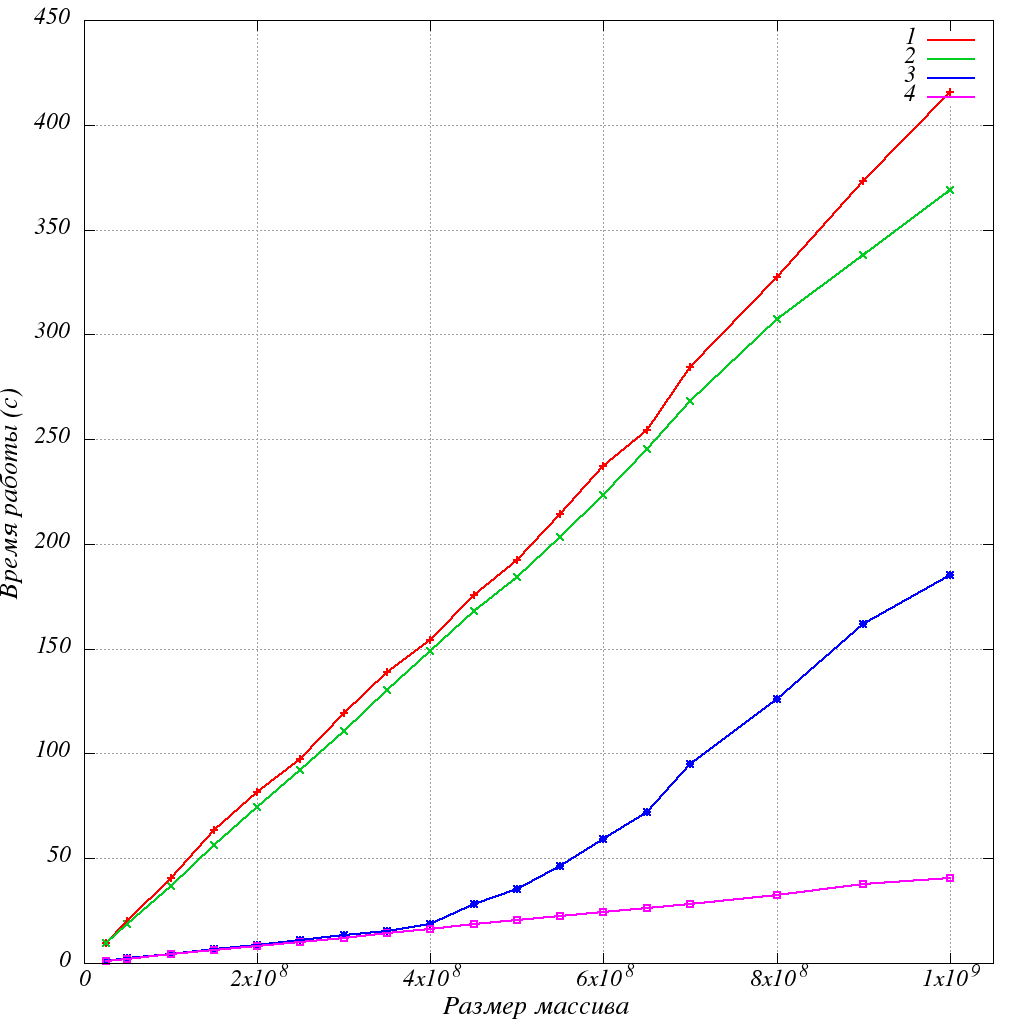
\includegraphics[width=1\linewidth]{graphics.png}}\\
\end{figure}


Тестирование на реальных моделях
\begin{tabular}{||l||c|c|c||}
\hline
\hline
& Время работы & Время работы & Ускорение \\
\hline
\hline
COORD & 0.028 & 0.003 & 9.33 \\
\hhline{~|-|-|-|}
ZCORN & 0.135 & 0.013 & 10.38 \\
\hline
COORD & 0.132 &  0.010 & 13.2 \\
\hhline{~|-|-|-|}
ZCORN & 12.819 & 0.982 & 13.05 \\
\hline
\hline
\end{tabular}


\section{Заключение}
\newpage

\newpage
\begin{thebibliography}{}

\bibitem{1} \textsc{Florian Loitsch}.
Printing Floating-Point Numbers Quickly and Accurately with Integers, 2004.
\bibitem{2} \textsc{Wojciech Mu\l a}.
SSE: conversion integers to decimal representation, 2011.


\end{thebibliography}

\end{document}
